\documentclass[a4paper,UTF8]{ctexart}

\usepackage{authblk}
\usepackage{setspace}
\renewcommand{\baselinestretch}{2.0} \usepackage[margin=1.25in]{geometry}
\usepackage{amsmath}
\usepackage{tabularx}
\usepackage{booktabs}
\usepackage{multirow}
\usepackage{makecell}
\usepackage{setspace}
\usepackage{siunitx}
\usepackage[backref]{hyperref}
\hypersetup{hidelinks} 
\usepackage{mathtools}
\usepackage{graphicx}
\usepackage{subfig} 
\graphicspath{{/home/ming/academic/tools/latex2word/tests/zh/multifigs}} 
\title{一个示例测试文档}

\author[1$\dag$]{作者A}
\author[1$\dag$]{作者B}
\author[1*]{作者C}
\author[1,2]{作者D}

\affil[1]{示例研究学院,示例大学}
\affil[2]{高级示例研究学院,示例大学}
\affil[*]{通讯作者:example.email@university.edu}
\affil[$\dag$]{这些作者对本文贡献相同。}

\begin{document}

\maketitle

\begin{abstract}
本文提供了一个学术论文的基本结构,其中包含用于测试表格、图片、公式和参考文献的示例。本文展示了常见的 LaTeX 命令和文档功能的示例。
\end{abstract}

\section{引言}

本文是一个测试示例,旨在帮助检查各种 LaTeX 排版技术,包括表格、图片和公式。在接下来的章节中,我们将展示这些功能。

\section{表格}

此部分包含一个简单的表格(表 \ref{tab:exampletable})。


\begin{table}[htbp]
    \centering
    \caption{
        一个参数示例表。
    }
    \label{tab:exampletable}
    \begin{tabular}{l}
    
\includegraphics[width=0.8\linewidth]{tab_exampletable.png}
    \end{tabular}
\end{table}


表 \ref{table3} 展示了一个更复杂的表格。


\begin{table}[htbp]
    \centering
    \caption{示例全球经济指标}
    \label{table3}
    \begin{tabular}{l}
    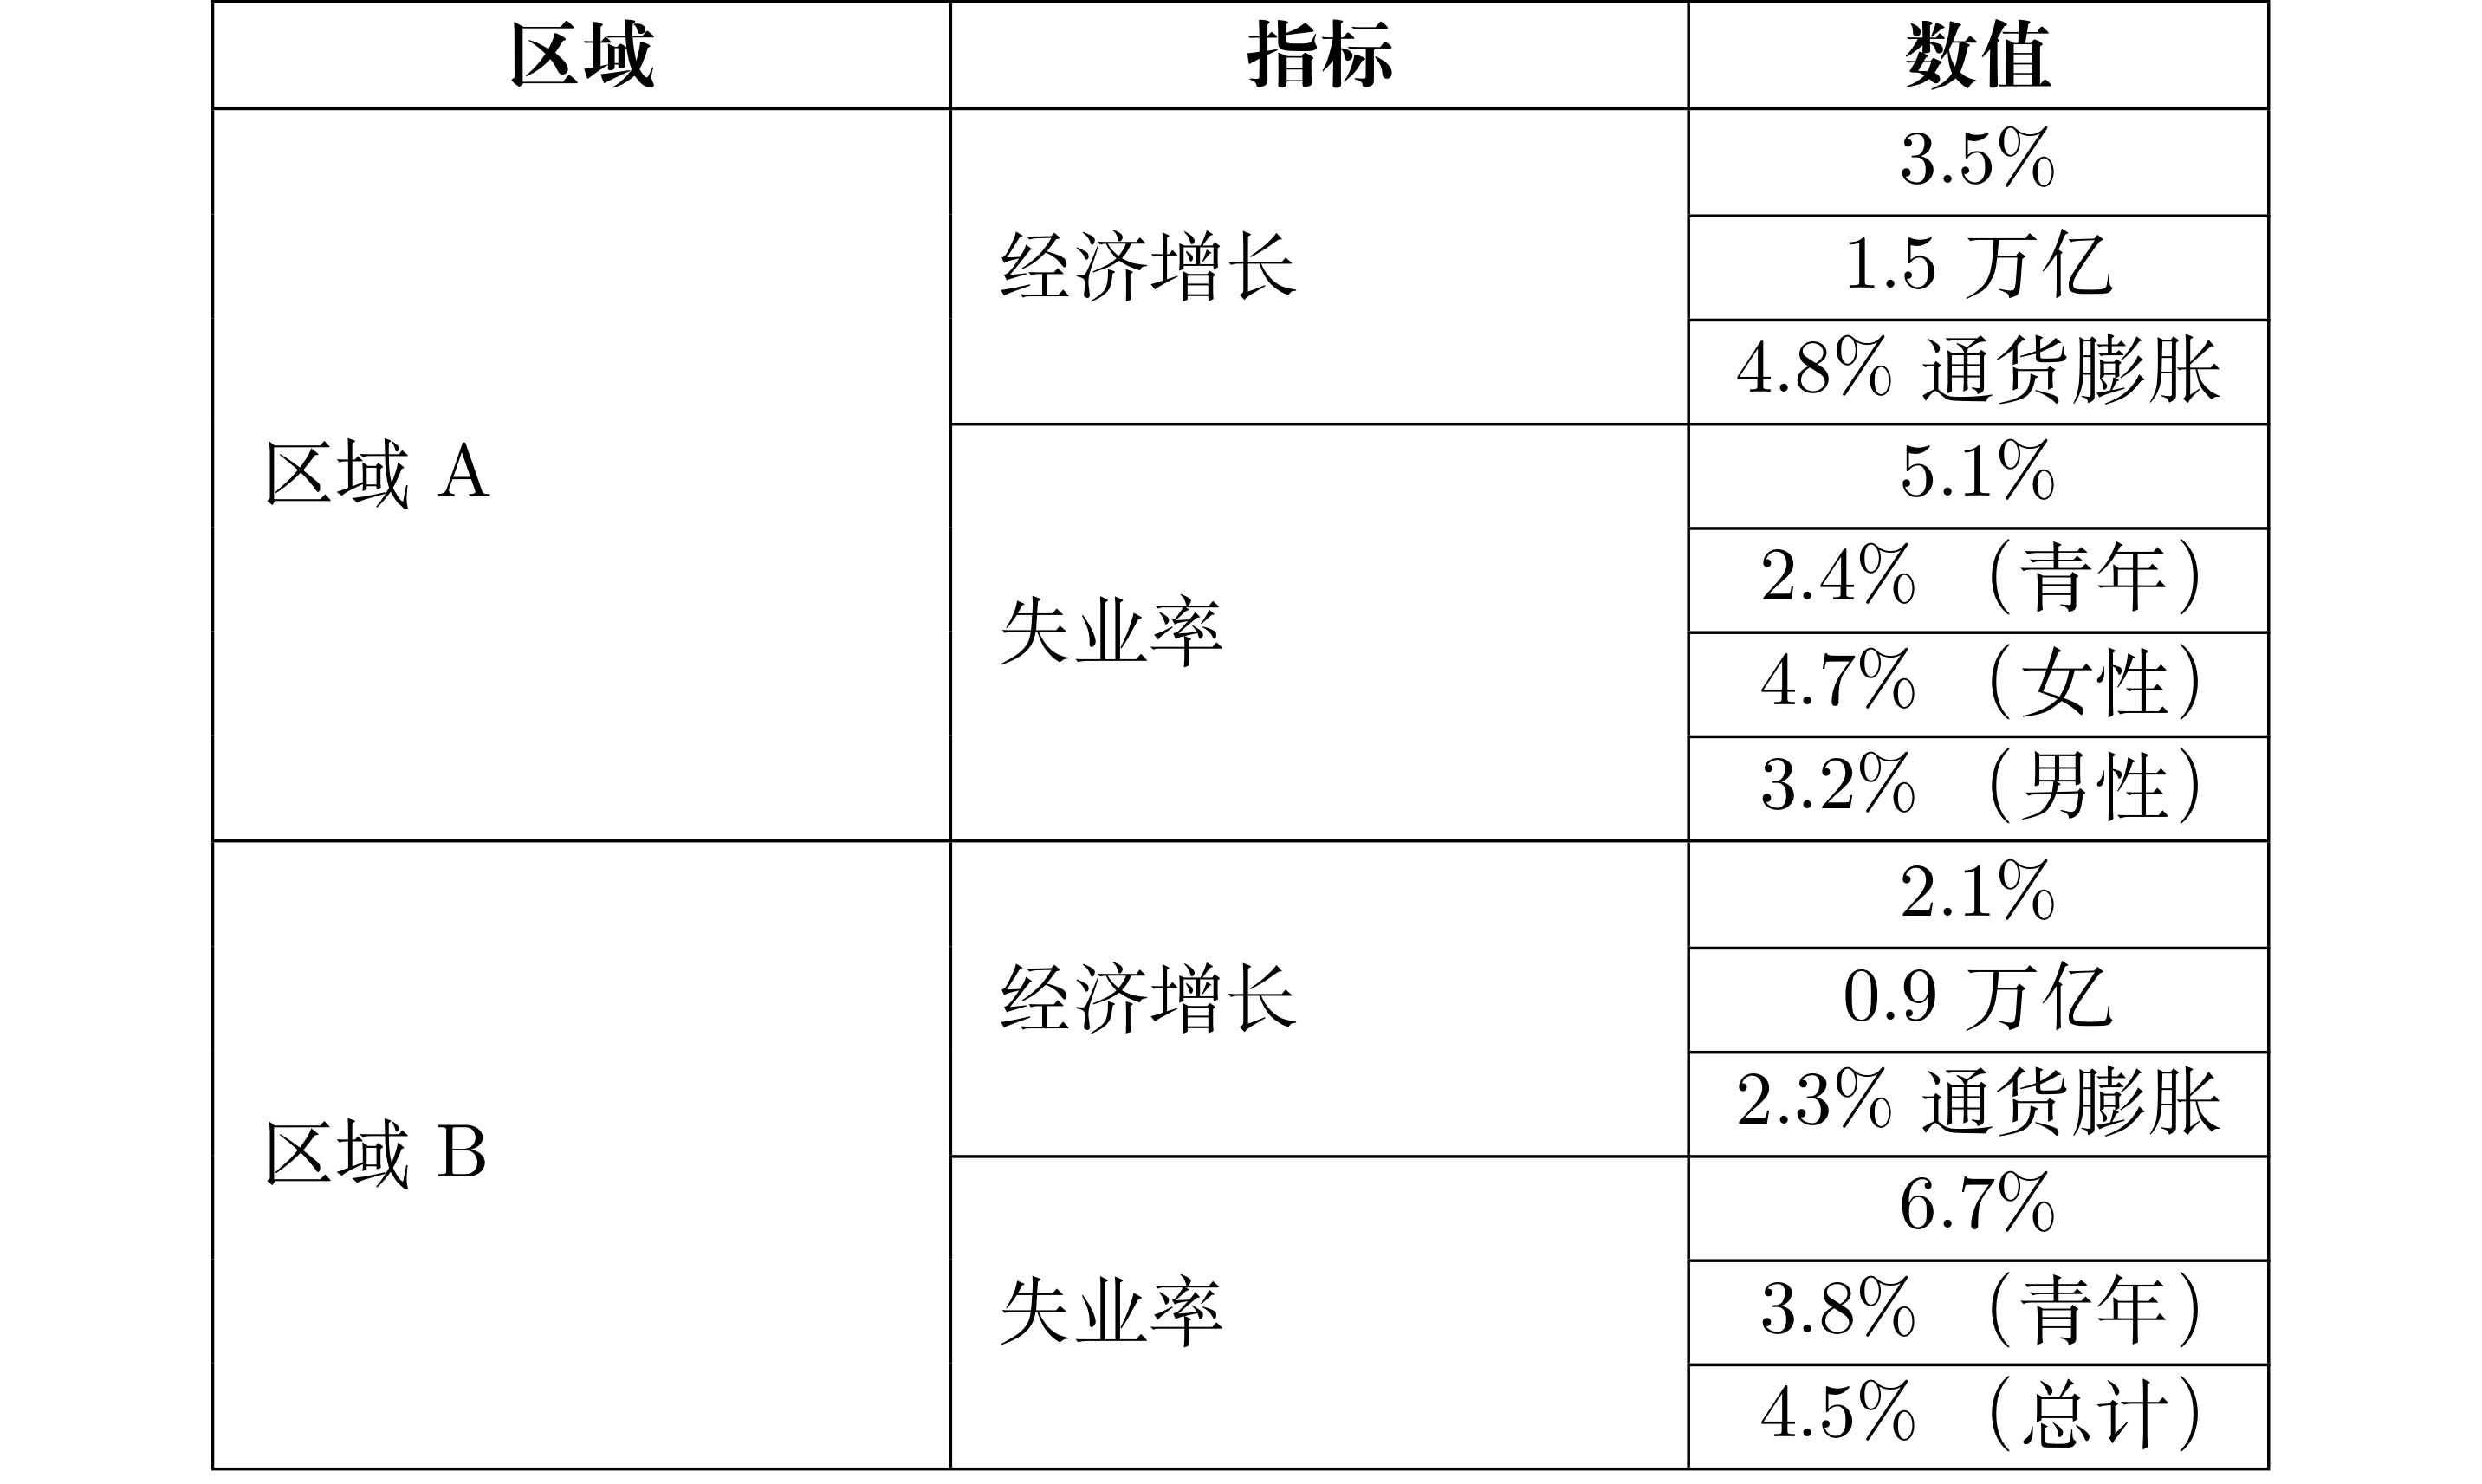
\includegraphics[width=0.8\linewidth]{tab_table3.png}
    \end{tabular}
\end{table}



\section{图片及其引用}

\subsection{示例图片}

下面是一个示例图片(图 \ref{multifig:multifig_examplefig}),展示了可能代表流程或概念的图示。


\begin{figure}[htbp]
    \centering
    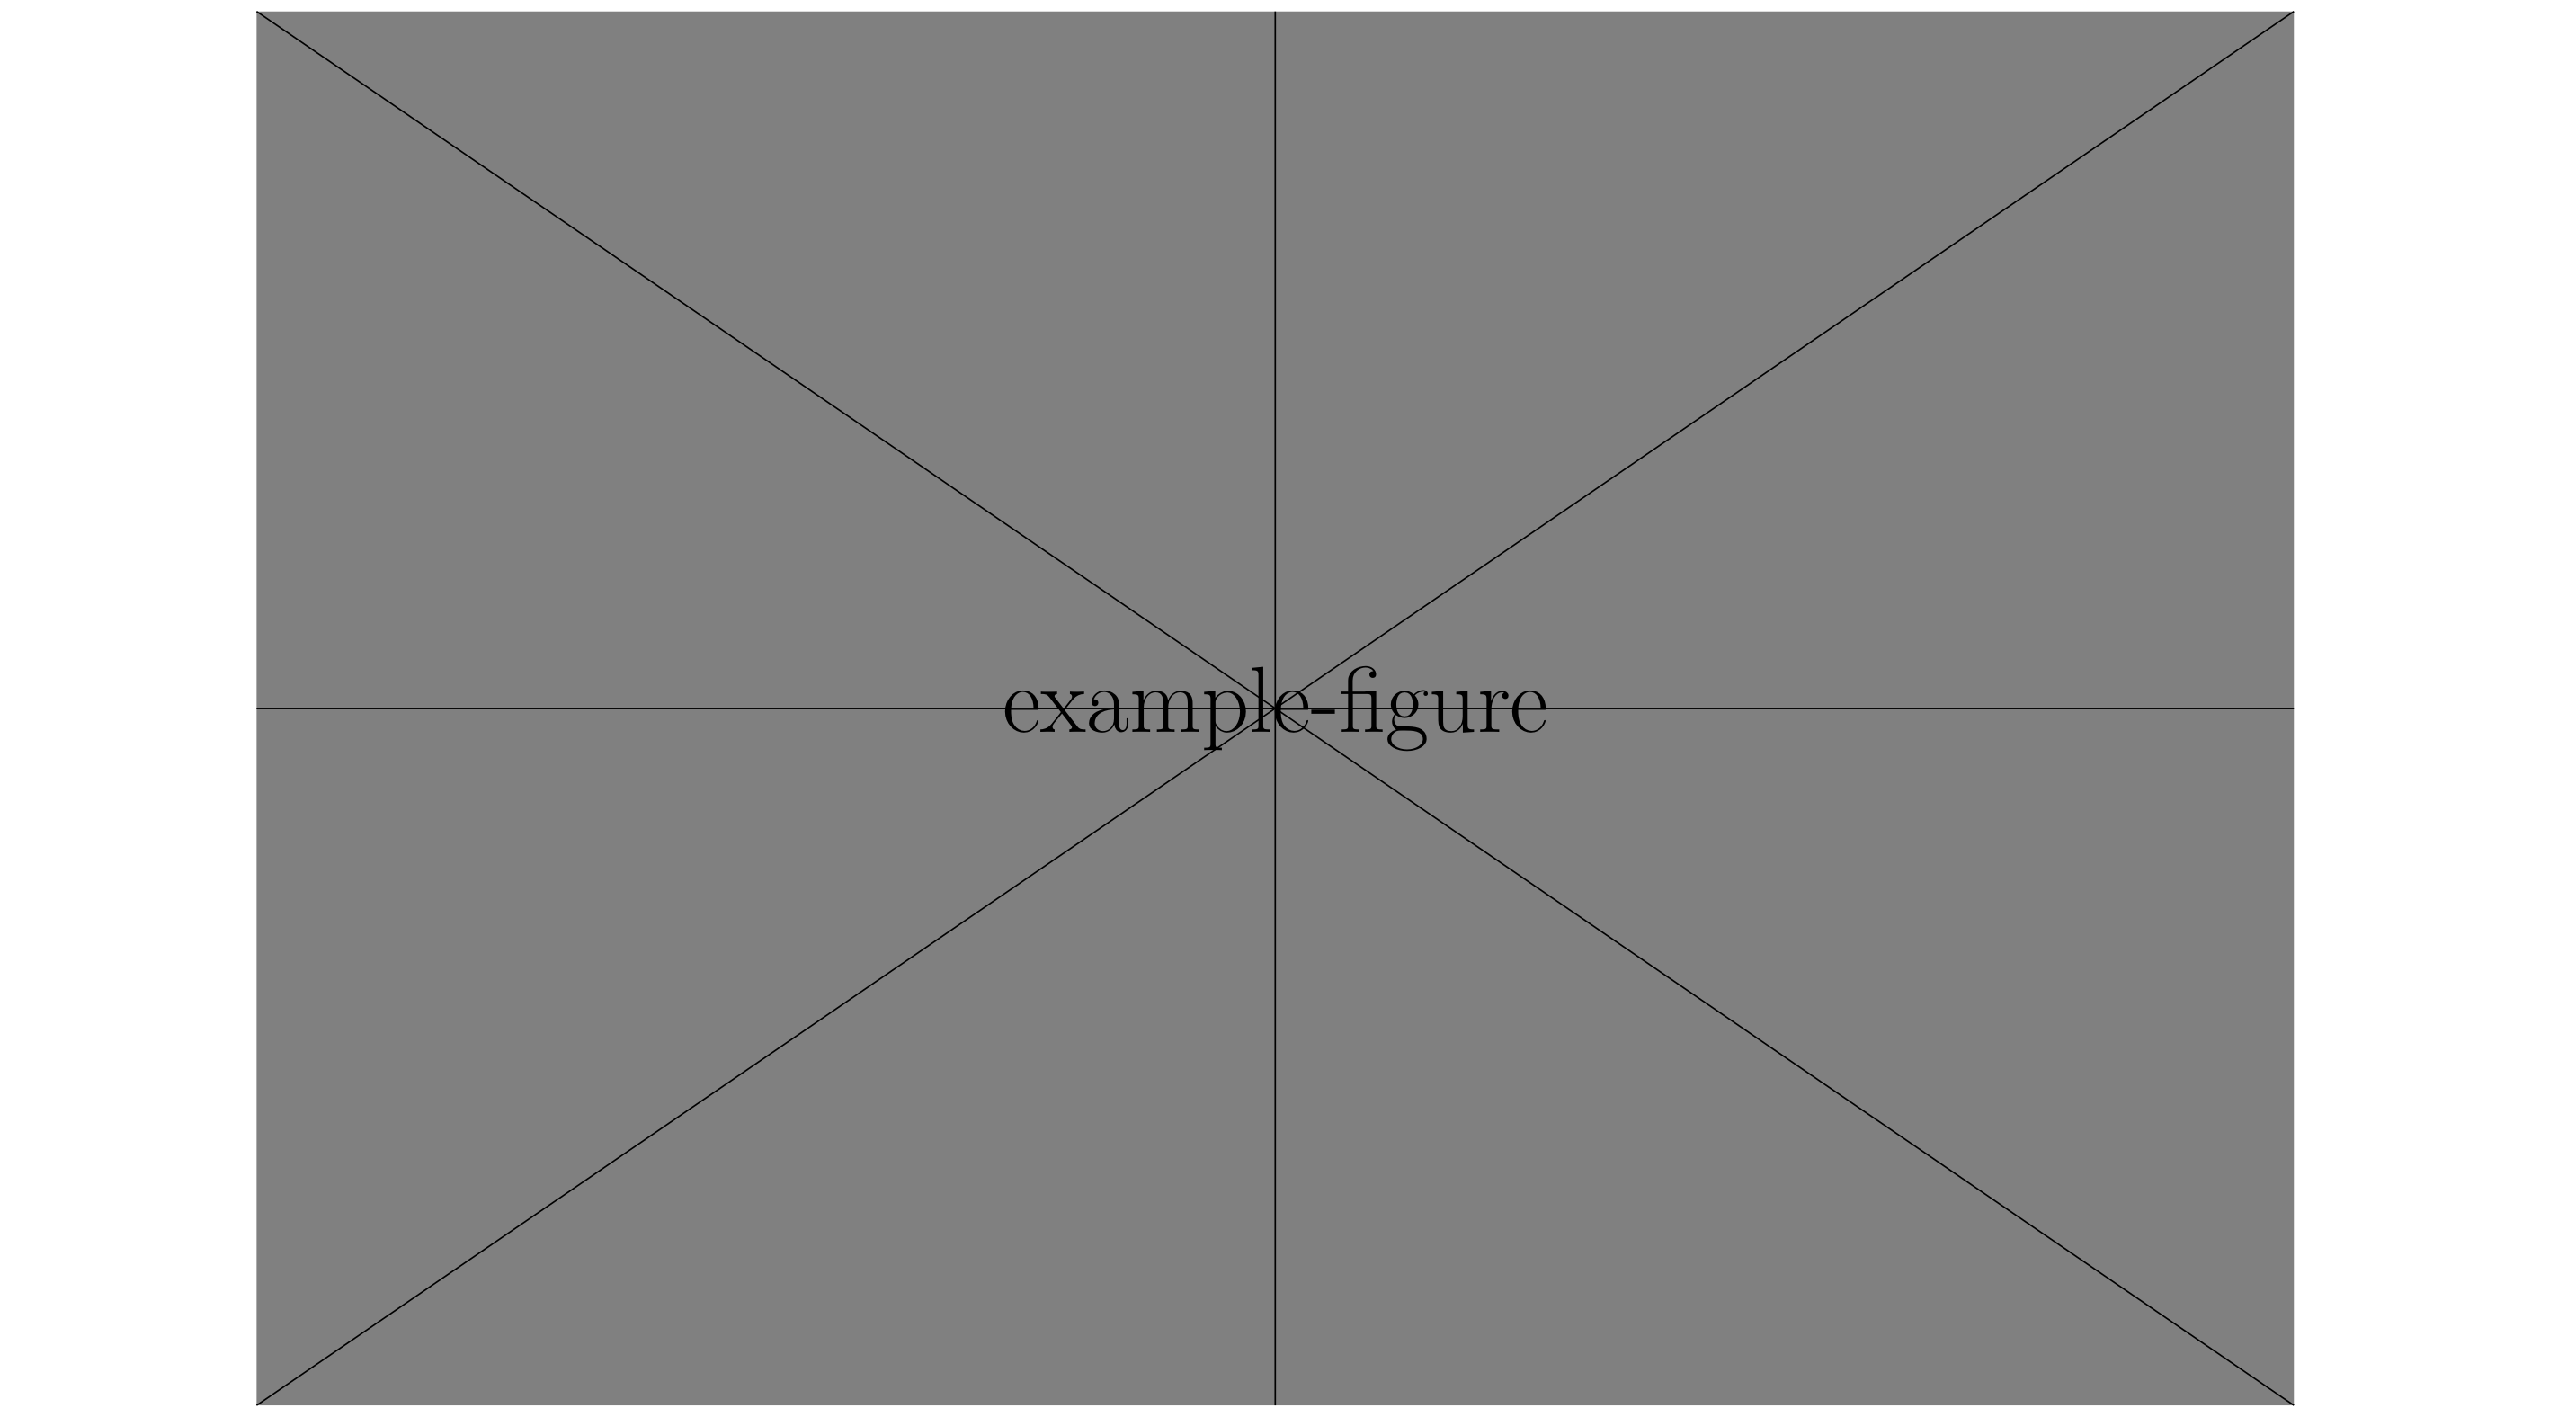
\includegraphics[width=0.8\linewidth]{multifig_examplefig.png}
    \caption{
        一个示例图片,展示了概念图。
    }
    \label{multifig:multifig_examplefig}
\end{figure}


\subsection{子图}

下面是一个包含 4 个子图的示例(图 \ref{multifig:multifig_examplesubfigures}),分别为图 \ref{multifig:multifig_examplesubfigures}(a)、图 \ref{multifig:multifig_examplesubfigures}(b)、图 \ref{multifig:multifig_examplesubfigures}(c) 和图 \ref{multifig:multifig_examplesubfigures}(d)。


\begin{figure}[htbp]
    \centering
    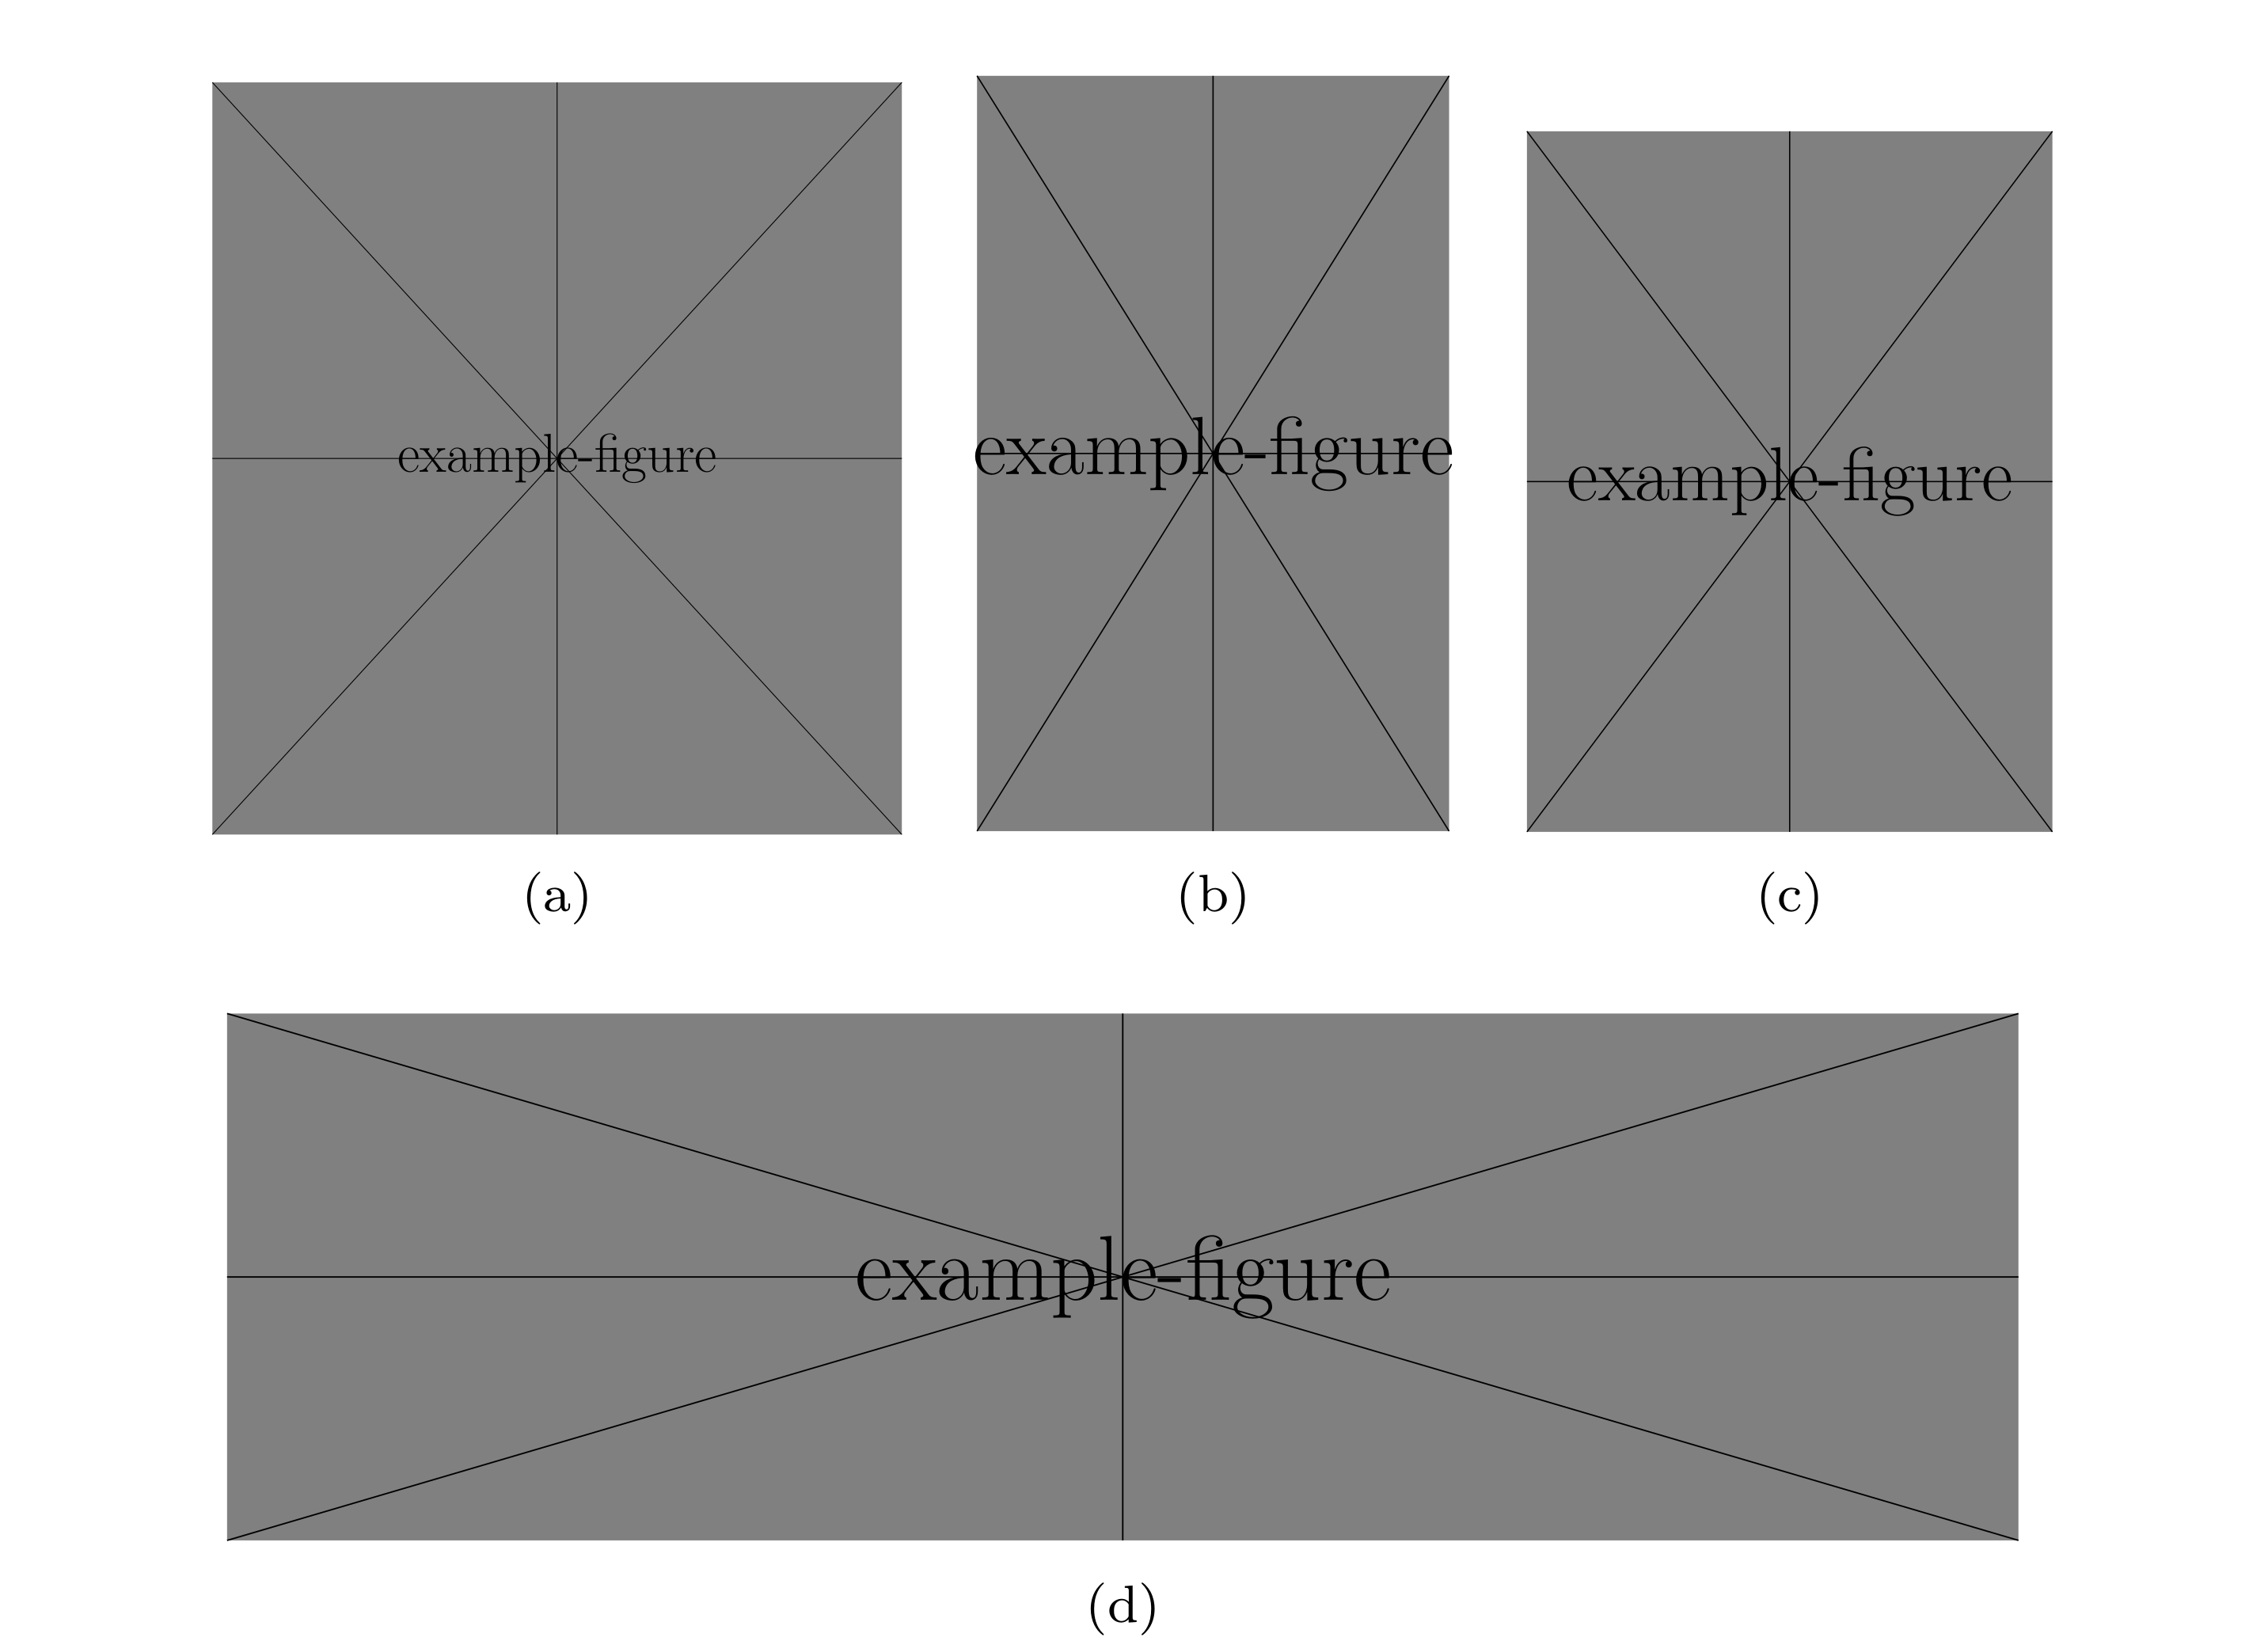
\includegraphics[width=0.8\linewidth]{multifig_examplesubfigures.png}
    \caption{
        示例子图 (a) 子图 1,(b) 子图 2,(c) 子图 3,(d) 子图 4。
    }
    \label{multifig:multifig_examplesubfigures}
\end{figure}


\section{公式和方程}

此部分包含一个公式的示例。关联矩阵的表达式如公式 \ref{eq:incidence} 所示:

\begin{align}\label{eq:incidence}
    a_{kl}=
    \begin{cases}
        1,  & \text{边 $l$ 离开节点 $k$},\\
        -1, & \text{边 $l$ 进入节点 $k$},\\
        0,  & \text{其他情况},
    \end{cases}
\end{align}
其中 $a_{kl}$ 是关联矩阵的元素,$k$ 是节点编号,$l$ 是边编号。

\section{参考文献}

此部分展示了如何引用参考文献 \cite{article1}。

\bibliographystyle{ieeetr}
\bibliography{../ref}

\end{document}
